\newpage
\subsection*{A4O3.3}
The rules for subtyping was added by the following Prolog facts and implications.

\begin{verbatim}
isTypeOf(X,B) :-
  isSubtypeOf(A,B),
  isTypeOf(X,A).


isSubtypeOf(bool,int).

isSubtypeOf(list(A),list(B)) :-
  isSubtypeOf(A,B).

/*
isSubtypeOf(A,C) :-
  isSubtypeOf(A,B),
  isSubtypeOf(B,C).
*/
\end{verbatim}
The last one is out commented as it produces an infinite loop, and since we will not need it we will just leave it out commented. The reason for the infinite loop is that when asking what dictionaries we can pass to \texttt{qsort} when sorting a list of booleans, outputting a list of integers, we first get one correct answer \texttt{ordInt}. Then we backtrack to try to find more solutions, and in that process we ask if \texttt{int} is a subtype of any type. We know it isn't, but because of the transitivity rule, the query will run infinitely, thus creating the infinite loop that prevents the program from terminating.

Now, in figure \ref{fig:boollist} is is determined how many different dictionaries that could be passed to \texttt{qsort'}, by issuing the following query.

\begin{figure}[h]
\centering
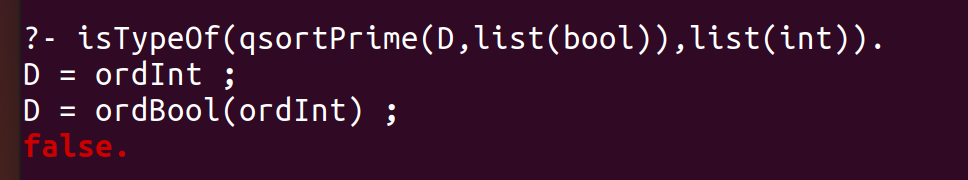
\includegraphics[width=0.8\textwidth]{O33.png}
\caption{Finding dictionaries for sorting a list of booleans into a list of ints.}
\label{fig:boollist}
\end{figure}

This means that there are two dictionaries that can be passed to \texttt{qsort'}. In this case both dictionaries work pefectly fine for sorting the list, but what if we didn't know whether we had a list of booleans or a list of integers? Then it might be smartest for us to use the \texttt{ordInt} dictionary, as that dictionary can sort both integers and booleans, and thus it is the more general dictionary of the two. Thus the dictionary the compiler should choose would be \texttt{ordInt}.
